\newpage
\section{Auswertung}
\label{sec:auswertung}
\subsection{Landefaktoren}
Um optimale Ergebnisse zu erzielen muss zunächst die vertikale Komponente des Erdmagnetfeldes komepensiert werden da diese einen störenden Offset in den Daten verursacht.
Dafür wird, wie in Abschnitt \ref{sec:durchfuerung} beschrieben, das Magnetfeld der vertikale Spule solange varriert bis sich drei schmaller Peaks zeigen.
Der Größte davon korrespondiert zu der vollen Komepensation des Magnetfelds in eine Richtung.
Die anderen Peaks treten dann auf wenn die Zeeman-Aufspaltung gleich der RF-Spulen Energie ist.
Es wird die B-Feld Stärke verwendet bei der die Peaks am schmallsten sind.
Dies wird bei einem Wert von $B_\text{v} = \SI{3.45e-5}{\tesla}$ erreicht.
Danach wird mit Hilfe einer horizontalen Sweep Spule die Magnetfeld Stärke in dieser Raumrichtung geändert.
Die horizontale B-Feldstärke in den Peaks wird dann gegen die angelegte RF-Spulelenfrequenz geplottet.
Der resultierende Plot ist in Abbildung \ref{fig:lande} zu sehen.
Da beiden Isotope unterschiedliche Landefaktoren haben unterscheidet sich auch die Steigung der Geraden die durch das Auftragen der $B$ und $f$ Werte entsteht.
Um nun das Erdmagnetfeld in Horizontal Richtung zu bestimmen wird für beide Isotope eine Ausgleichsgerade nach der Gleichung 
\begin{equation}
    B(f) = a\cdot f + b
\end{equation}
angefertigt.
Die berechneten Parameter für das erste Isotop sind dabei 
\begin{align*}
    a_\text{Iso1} & = \SI{0.495(7)}{\tesla\Hz} \\
    b_\text{Iso1} & = \SI{2.23(13)e-05}{\tesla}
\end{align*}
und die für das zweite Isotop sind
\begin{align*}
    a_\text{Iso2} &= \SI{0.3317(17)}{\tesla\Hz}\\ 
    b_\text{Iso2} &= \SI{2.34(7)e-05}{\tesla} \, .
\end{align*}
Der Wert $b$ gibt nun die jeweilige horizontale Erdmagnetfeldstärke an.
\begin{figure}
    \centering
    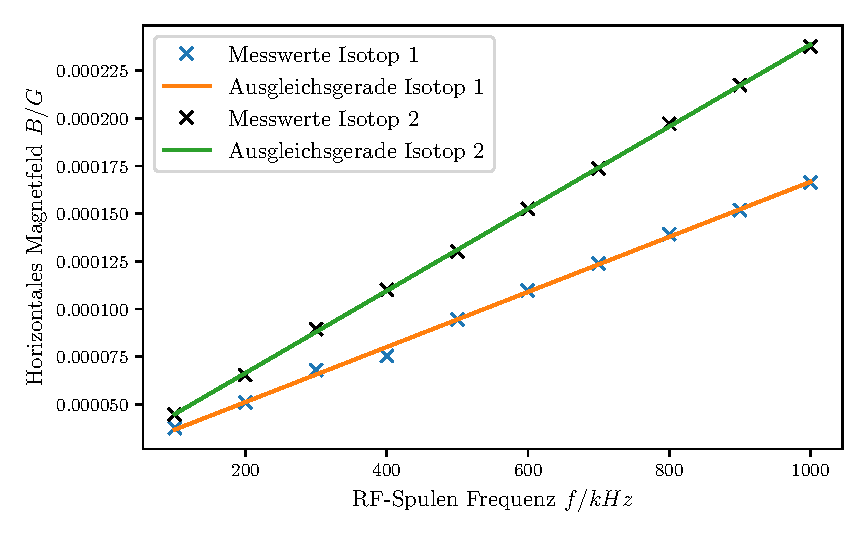
\includegraphics[width=\textwidth]{content/plots/landefaktor.pdf}
    \caption{Die Abbildung zeigt die B-Felder der negativen Peaks beider Isotope die gegen die RF-Spulelenfrequenz aufgetragen wird.
    Es ist zu erkennen das die resultierenden Geraden unterschiedliche Steigungen haben.
    In der Abbildung sind zudem zwei Ausgleichsgerade zu sehen die in die Messwerte beider Isotope hineingesetzt werden.}
    \label{fig:lande}
\end{figure}
Aus den Steigungen $a_\text{Iso1}$ und $a_\text{Iso2}$ können nun die beiden Landefaktoren der Isotope berechnet werden.
Dafür wird Gleichung \eqref{eq:zeeman_frequenz} genutzt wodurch sich die Landefaktoren
\begin{align*}
    g_\text{Iso1} &= \SI{0.4950(70)}{}\\
    g_\text{Iso2} &= \SI{ 0.3317(17)}{}
\end{align*}
ergeben.
\subsection{Kernspin}
Aus den zuvor berechneten Landefaktoren kann nun der Kernspin beider Isotope bestimmt werden.
Da bei den genutzt Isotopen gilt, dass 
\begin{align*}
    J, S &= \frac{1}{2}\\
    L &= 0
\end{align*}
kann mithilfe der Gleichung \eqref{eq:landefaktor} der Kernspin werden, da dies die letzte unbekannte Größe ist.

So ergeben sich für die oben genannten Werte des Landefaktors die Kernspins 
\begin{align*}
    I_\text{Iso1} &= \SI{1.522(30)}{}\\
    I_\text{Iso2} &= \SI{2.515(15)}{} \, .
\end{align*}

In Quelle \cite{pdf_anleitung} ist angeben, dass das Isotop {$^{85}\text{Rb}$ einen Kernspin von $\frac{5}{2}$} und das Isotop $^{87}\text{Rb}$ einen Kernspin von $\frac{3}{2}$ hat.
Damit erschließt sich, dass Isotop 1  $^{87}\text{Rb}$ ist und Isotop 2 $^{85}\text{Rb}$ entspricht.

\subsection{Isotopenverhältnis}
Für die Bestimmung des Isotopenverhältnis wird die Abbildung \ref{fig:isotop} in 'inkscape' \cite{Inkscape} eingefügt um die Tiefe der Peaks in Anzahl von Pixeln zu zählen.

\begin{figure}
    \centering
    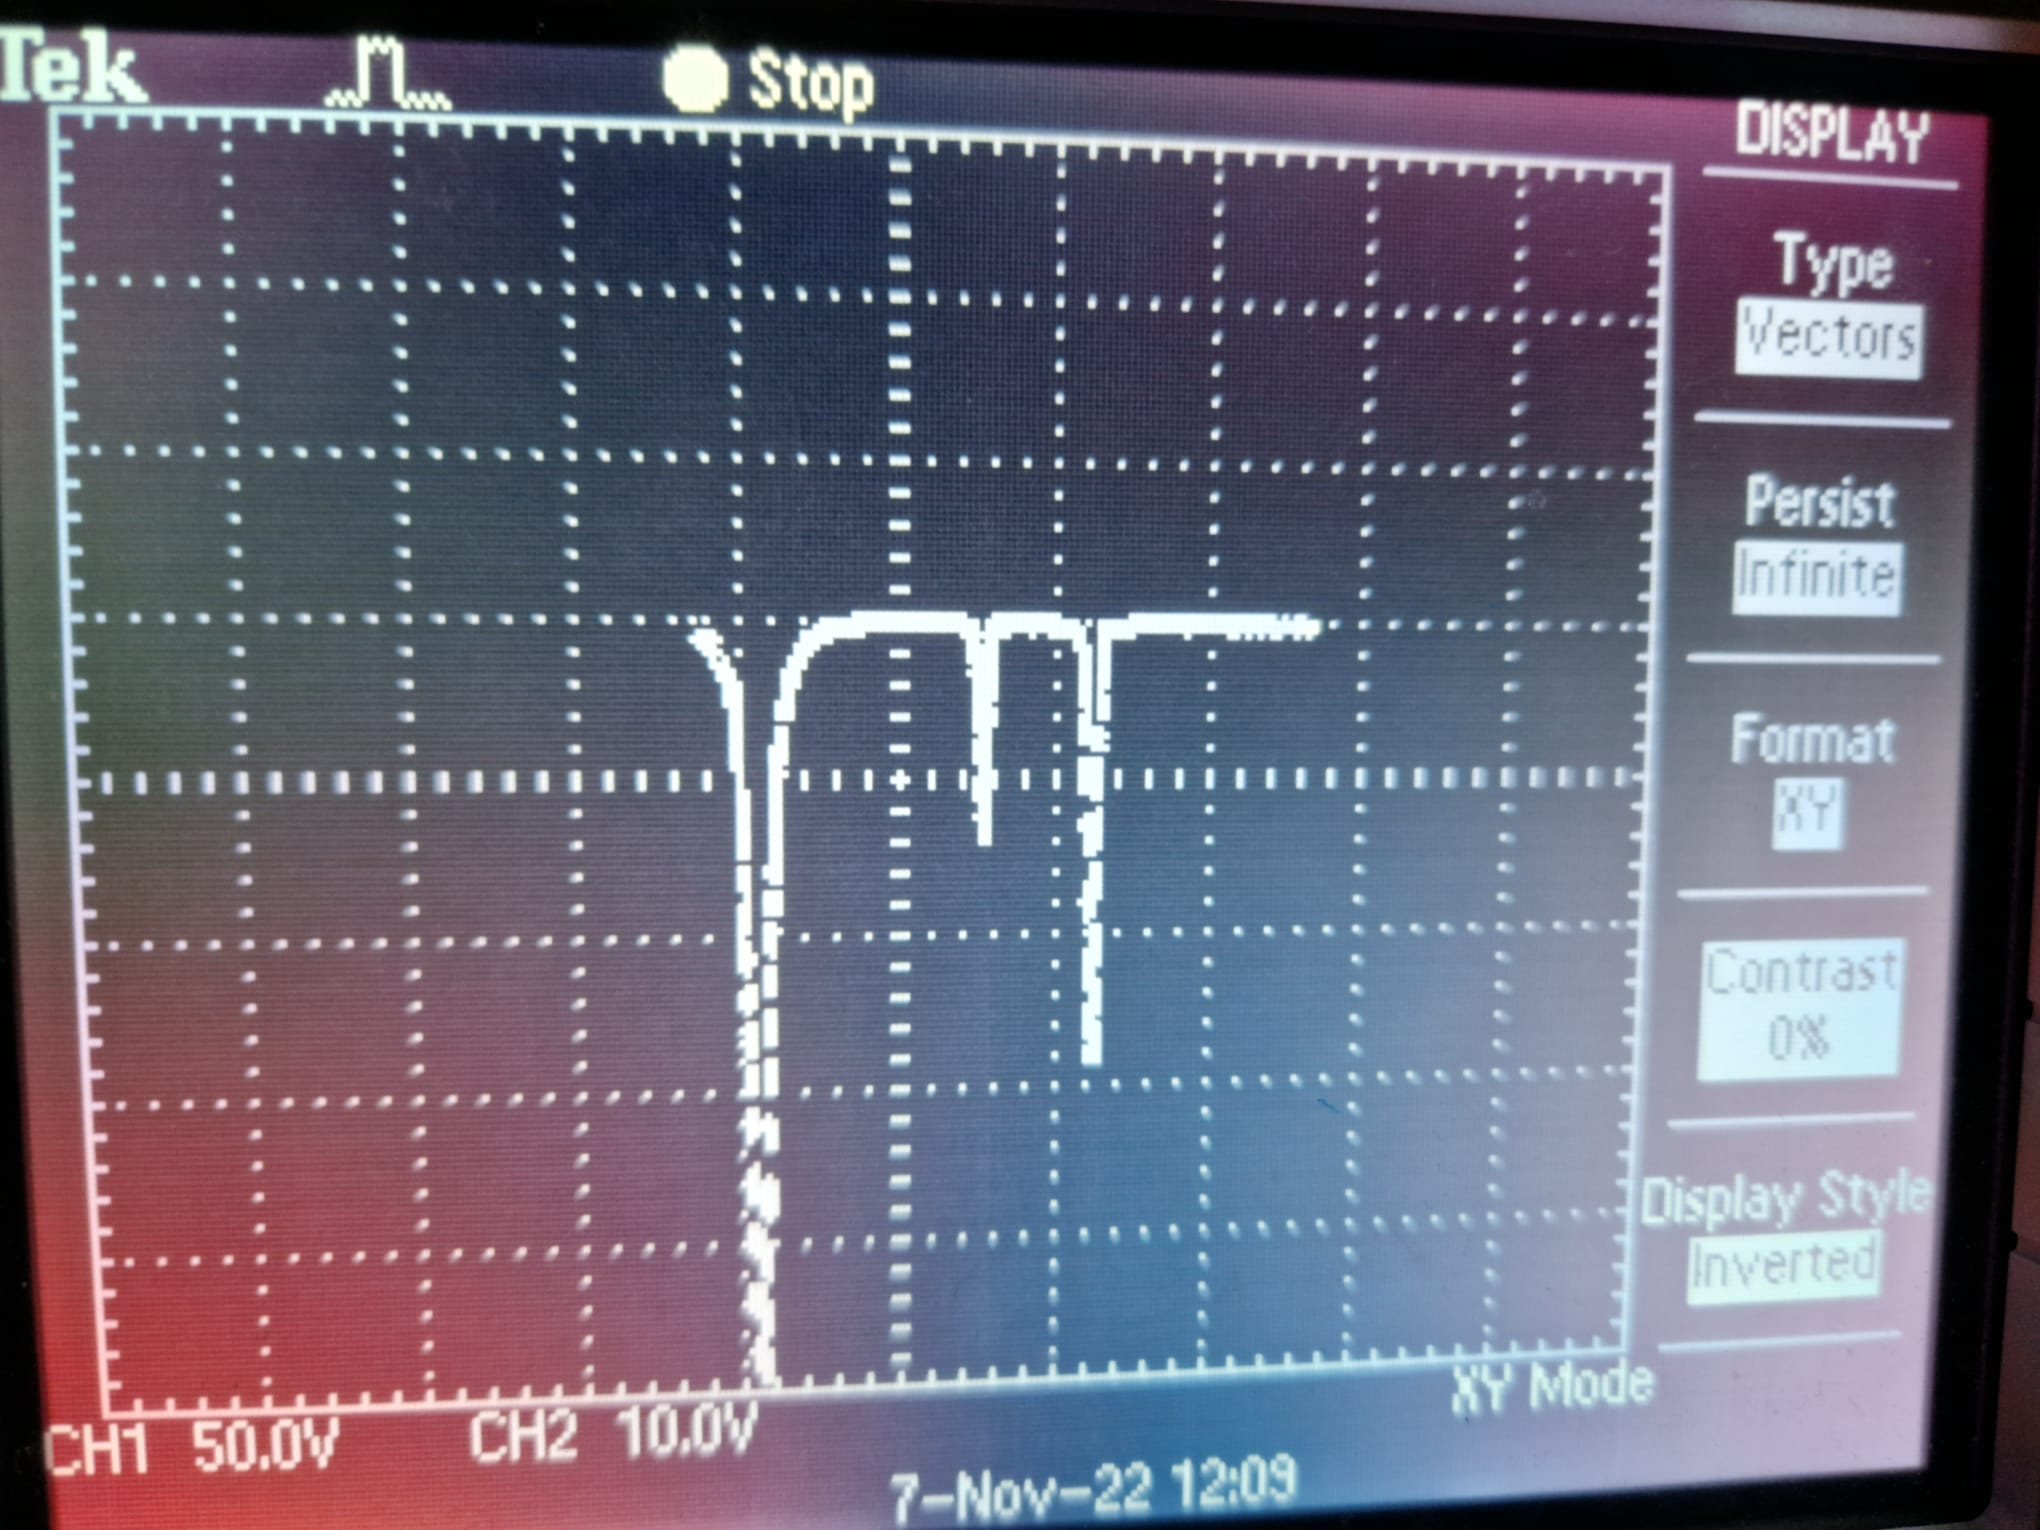
\includegraphics[width=0.5\textwidth]{Data/isotope.jpeg}
    \caption{Ein Foto der Messung die mit einem Oszilloskop aufgenommen wird.
    Diese trägt das angelegte Magnetfeld gegen den Strom der Photodiode auf.
    Es sind drei negative Peaks zu sehen.
    Von links nach rechts korrespondieren diese zu dem Nulldurchgang des angelegte Magnetfeldes, dem 1. Isotop und dem zweiten Isotop.}
    \label{fig:isotop}
\end{figure}
Für den linken negativen Peak wird eine Anzahl von $61.356$ Pixeln und für den Rechten $118.71$ Pixel gezählt.
Damit stellt sich ein Isotopenverhältnis von 
\begin{align*}
    ^{87}\text{Rb} \, &\widehat{=}\, 34.07\% \\
    ^{85}\text{Rb} \, &\widehat{=}\, 65.92\%
\end{align*}
ein.

\subsection{Quadraitsche Zeemanaufspaltung}
Um die Stärke der maximalen quadratischen Zeemanaufspaltung bei gegebenen Versuchsaufbau abzuschätzen wird bei der Resonanzfrequenz von $\SI{100}{\k\Hz}$ das größt mögliche Magnetfeld genutzt.
Aus Quelle \cite{pdf_anleitung} ist zu entnehmen, dass für $^{85}\text{Rb}$ $m_\text{F} = 3$ ist und für $^{87}\text{Rb}$ $m_\text{F} = 2$ ist.
Daraus kann nun mit Gleichung \eqref{eq:zeemanaufspaltung} die maximale Zeemanaufspaltung berechnet werden.
Die Aufspaltungen zu den jeweiligen Magnetfeldstärken sind
\begin{align*}
    \Delta E_\text{Iso1} = \SI{4.77(7)}{\eV} & B=\SI{0.1665}{\m\tesla} \\
    \Delta E_\text{Iso2} = \SI{4.557(23)}{\eV} & B=\SI{0.2377}{\m\tesla}  \, .
\end{align*}

\subsection{Rabioszillation}
Die Messwerte für diesen Abschnitt werden gemäß das Ablaufs der in Abschnitt \ref{sec:rabi} beschrieben wird, aufgenommen.
Danach wird die Periodendauer $T$ gegen die RF-Amplitude $A_0$ aufgetragen.
Der resultierende Plot ist in Abbildung \ref{fig:rabi} zu sehen.
\begin{figure}
    \centering
    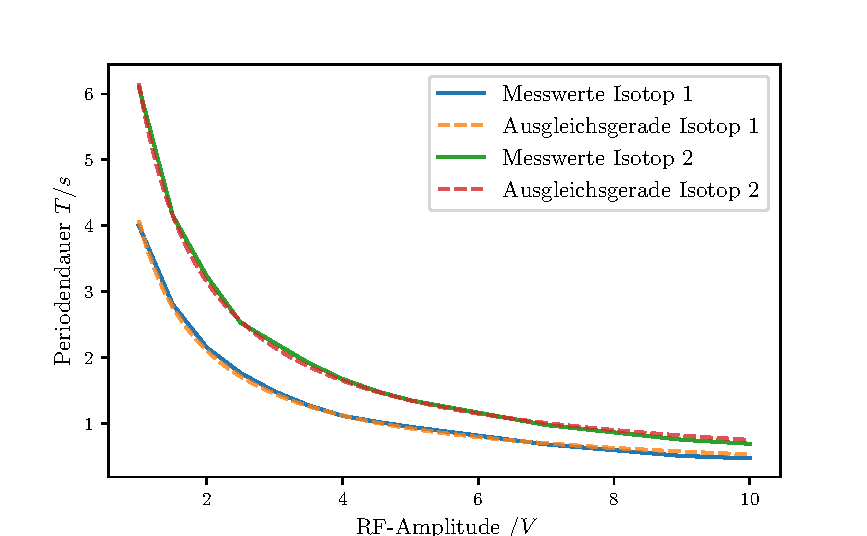
\includegraphics[width=\textwidth]{content/plots/periodendauer.pdf}
    \caption{Die Periodendauer der Rabioszillation wird gegen die angelegte RF-Amplitude aufgetragen.
    Zudem wird eine Ausgleichsrechung durchgeführt dessen Fit ebenfalls in der Grafik zu sehen ist.}
    \label{fig:rabi}
\end{figure}
An die Messwerte beider Isotope wird ein Fit gemäß der Gleichung 
\begin{equation*}
    T(A_0) = a + \frac{b}{A_0}
\end{equation*}
angepasst.
Die berechneten Parameter für Isotop 1 sind 
\begin{align*}
    a_\text{Iso1} &= \SI{0.132(23)e-3}{\ms}\\
    b_\text{Iso1} &= \SI{3.94(5)e-3}{\V\ms} \, .
\end{align*}
Für Isotop 2 ergeben sich die Parameter 
\begin{align*}
    a_\text{Iso2} &= \SI{0.145(26)}{\ms}\\
    b_\text{Iso2} &= \SI{6.01(6)}{\V\ms} \, .
\end{align*}
Der gefragt Quotient aus $\frac{b_\text{Iso2}}{b_\text{Iso1}}$ kann nun berechnet werden.
Dieser beträgt 
\begin{align*}
    \frac{b_\text{Iso2}}{b_\text{Iso1}} &= \SI{1.525(26)}{} \, .
\end{align*}
\begin{figure}
    \centering
    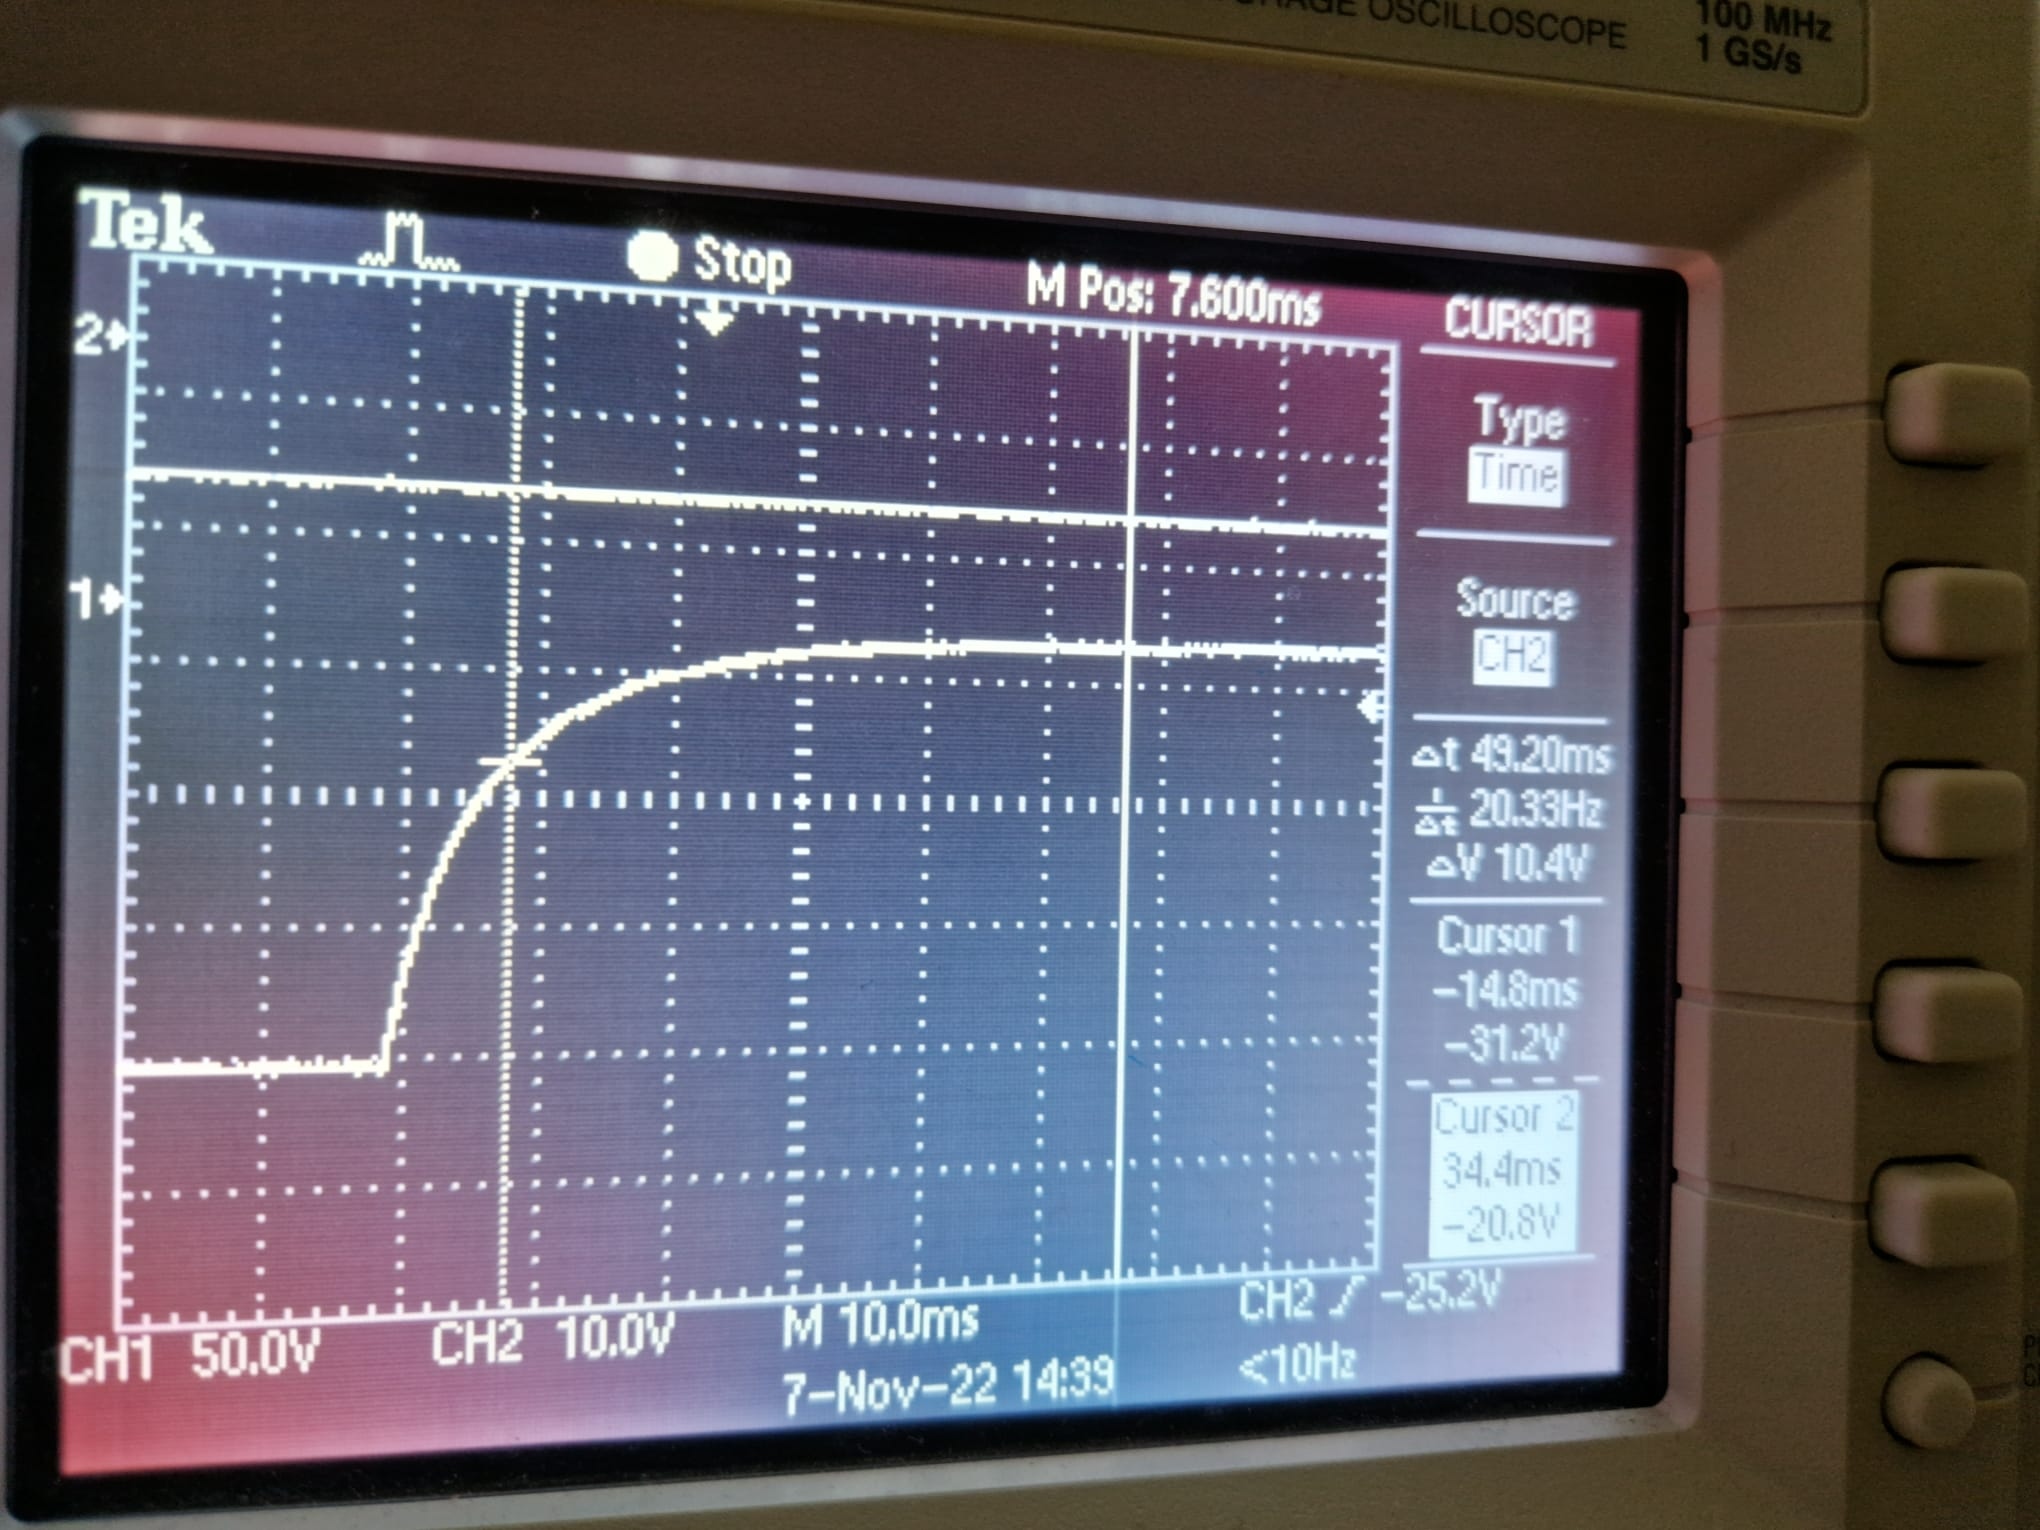
\includegraphics[width=0.5\textwidth]{Data/anstieg.jpeg}
    \caption{Der Anstieg des Photodioden-Stroms nach Einschalten des RF-Feldes.
    Es ist der typische exponentielle Verlauf zu erkennen.}
\end{figure}